\chapter{Introduction to Digital Systems}\label{cha:intr-digit-syst}

\setcounter{section}{8}

\clearpage

\section{From Binary Logic (Mathematics) to Logic Gates (Circuits)}\label{sec:from-binary-logic}

From what we have studied in Discrete Mathematics, we have the
following basic three logic functions:

\hfil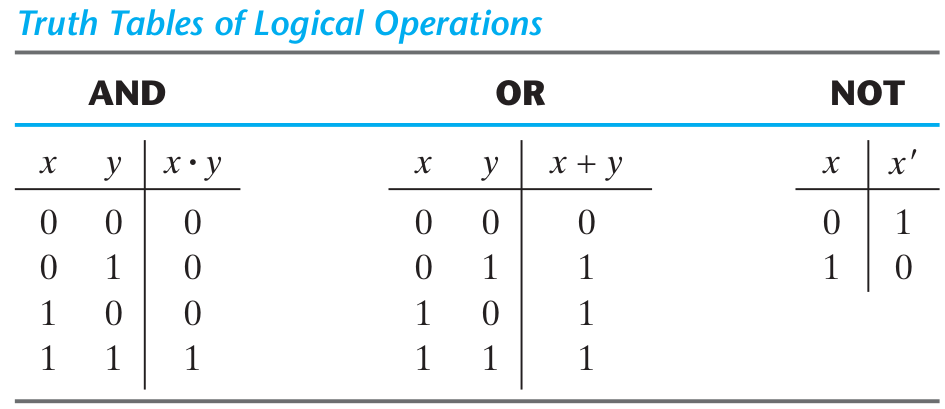
\includegraphics[width=.7\textwidth]{../Graphics/Ch01Art29.png}\hfil

\clearpage

\hfil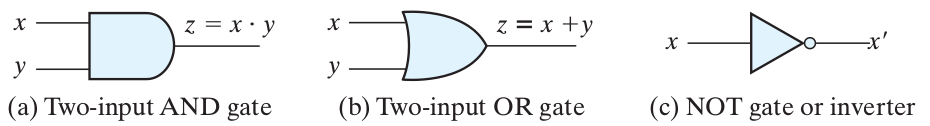
\includegraphics[width=\textwidth]{../Graphics/Ch01Art30b.png}\hfil

\clearpage

\hfil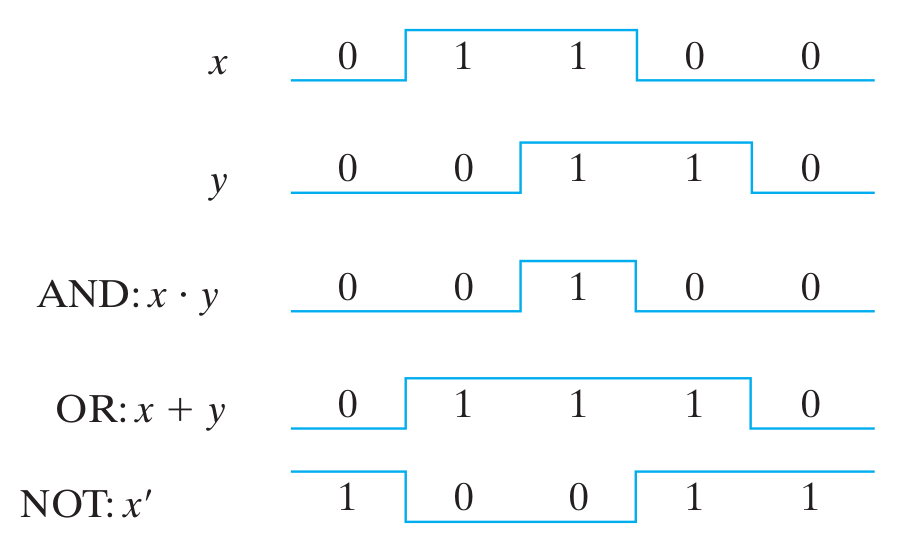
\includegraphics[width=\textwidth]{../Graphics/Ch01Art31a.png}\hfil

\clearpage

\hfil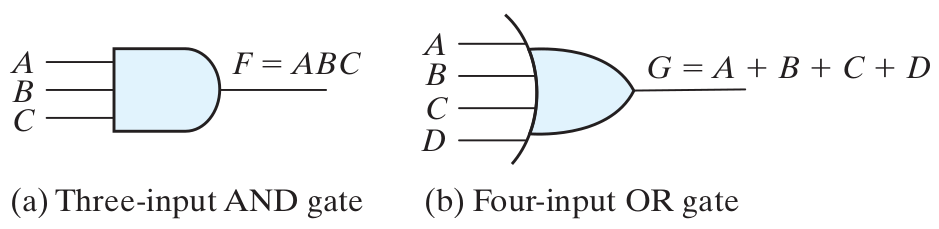
\includegraphics[width=\textwidth]{../Graphics/Ch01Art31b.png}\hfil

\clearpage

\hfil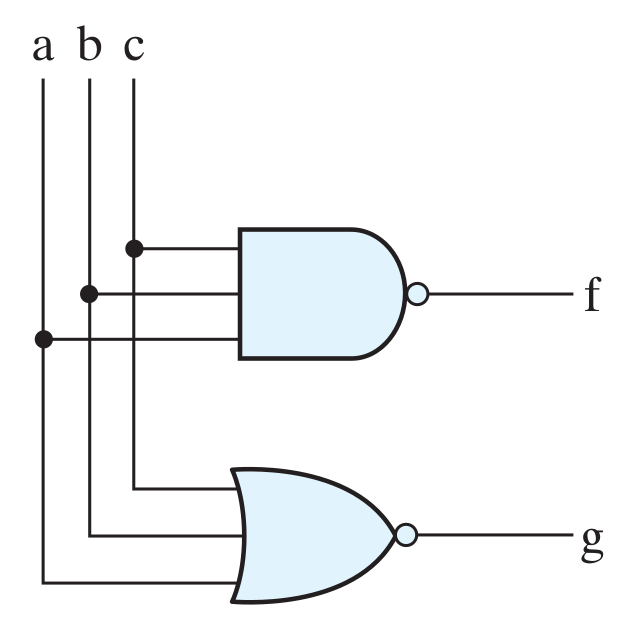
\includegraphics[width=.7\textwidth]{../Graphics/Ch01Art34a.png}\hfil



\clearpage

\section*{Revisiting Course Objectives}\label{sec:revis-course-object}

\subsection*{Theory (hands on paper)}\label{sec:theory-hands-paper}

\hfil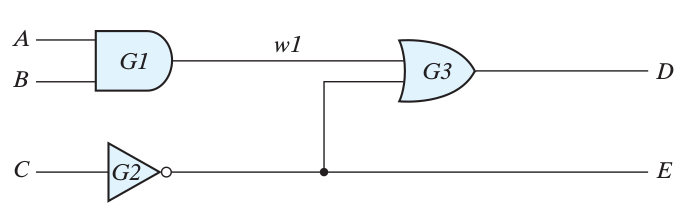
\includegraphics[width=.5\textwidth]{../Graphics/Ch03Art42.png}\hfil


\subsection*{Simulation using Verilog}\label{sec:simul-using-veril}

\begin{lstlisting}
// Verilog model: Simple_Circuit
module Simple_Circuit (A, B, C, D, E);
  output D, E;
  input  A, B, C;
  wire	 w1;
  
  and 	 G1 (w1, A, B); //Optional gate instance
  not	 G2 (E, C);
  or	 G3 (D, w1, E);
endmodule
\end{lstlisting}

\subsection*{Hardware Implementation}\label{sec:hardw-impl}

\clearpage
\refstepcounter{PageDummyCounter}\label{sec:hardw-impl-5}
\hfil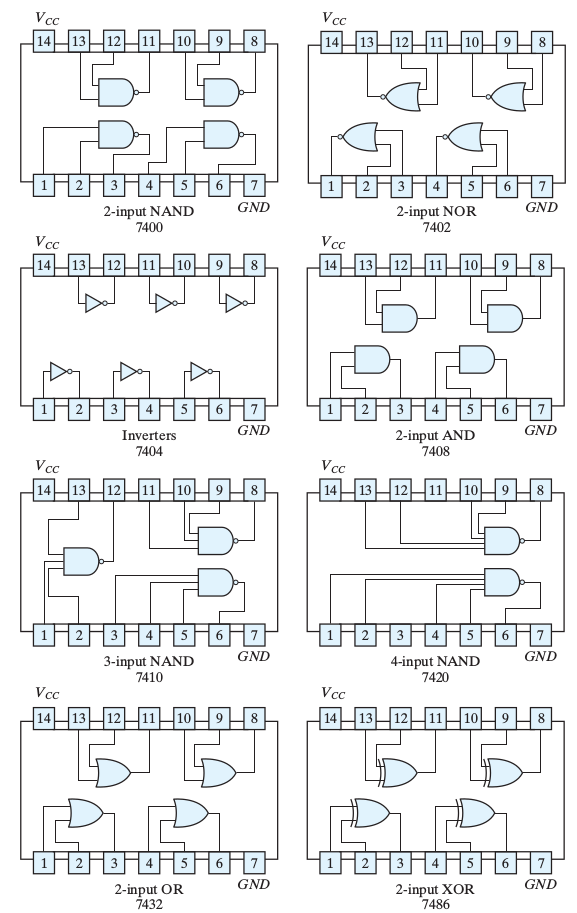
\includegraphics[height=\textheight]{../Graphics/Ch11Art513.png}\hfil

%%% Local Variables:
%%% mode: latex
%%% TeX-master: "../LectureNotesCS221"
%%% End:
